\documentclass[tikz, border=0.15mm]{standalone}
\usepackage{ytableau,tikz,varwidth}
\usetikzlibrary{calc}
\usepackage{mathrsfs}
\newcommand{\typeA}{magenta!65}
\newcommand{\typeB}{blue!75}
\newcommand{\typeC}{green!65}

\begin{document}
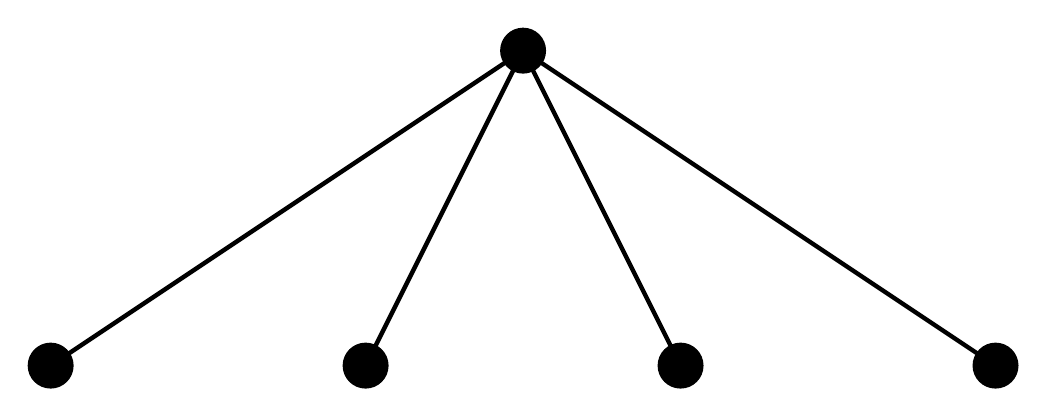
\begin{tikzpicture}[inner sep=0in,outer sep=0in]
	draw \node[circle, draw = black, ultra thick, minimum size=15pt, fill] at (6,0) (1) {A};
	draw \node[circle, draw = black, ultra thick, minimum size=15pt, fill] at (0,-4) (x_1) {};
	draw \node[circle, draw = black, ultra thick, minimum size=15pt, fill] at (4,-4) (x_2) {};
	draw \node[circle, draw = black, ultra thick, minimum size=15pt, fill] at (8,-4) (x_3) {};
	draw \node[circle, draw = black, ultra thick, minimum size=15pt, fill] at (12,-4) (x_4) {};
	
	\draw[black,ultra thick] (1)--(x_1);
	\draw[black,ultra thick] (1)--(x_2);
	\draw[black,ultra thick] (1)--(x_3);
	\draw[black,ultra thick] (1)--(x_4);
\end{tikzpicture}
\end{document}